\documentclass[a4paper]{exam}

\usepackage{amsmath,amssymb, amsthm}
\usepackage{geometry}
\usepackage{graphicx}
\usepackage{hyperref}
\usepackage{titling}
\usepackage{tikz}
\usepackage{tikz-qtree}
\usepackage{framed}

% \graphicspath{{images/}}


\newtheorem{definition}{Definition}
\newtheorem{theorem}{Theorem}
\newtheorem{corollary}{Corollary}
\newtheorem{axiom}{Axiom}
\theoremstyle{claim}
\newtheorem{claim}{Claim}

% Header and footer.
\pagestyle{headandfoot}
\runningheadrule
\runningfootrule
\runningheader{CS/MATH 113 2026}{Pset 10: Graphs}{\theauthor}
\runningfooter{}{Page \thepage\ of \numpages}{}
\firstpageheader{}{}{}

% \printanswers %Uncomment this line

\title{Problem Set 10: Graphs}
\author{Blingblong} % <=== replace with your student ID, e.g. xy012345
\date{CS/MATH 113 Discrete Mathematics\\Habib University\\Spring 2026}


% \qformat{{\large\bf \thequestion. \thequestiontitle}\hfill}
% \boxedpoints


\begin{document}
\maketitle      


\section*{Problems}
In the following problem set assume all the graphs are simple and finite unless specified otherwise.
\begin{questions}
  \question In parkour civilization everything is parkour. For some positive integer $m$ there are at most $2m+1$ houses at the parkour pro level of parkour civilization. From each house you can parkour to exactly $m$ other houses. Every parkour pro is sleeping inside a house. Tung Tung Tung Sahur wants to wake up all the parkour pros. For this he wishes to parkour to each of the houses in parkour civilization. By the help of Agent 5.5 he can teleport to any one house of his choice by then from there he would have to parkour to every other house he wishes to visit. Can Tung Tung Tung Sahur visit every house and wake up every parkour pro? Give a formal proof for your answer.
  \begin{figure}[h!]
    \centerline{\includegraphics[scale = 0.2]{tungtungtunsahur.png}}
    \caption{Tung Tung Tung Sahur \href{https://www.youtube.com/watch?v=HmIMmFAV4BY}{\url{https://www.youtube.com/watch?v=HmIMmFAV4BY}}}
  \end{figure}

  \begin{solution}
    % Enter your solution here.
  \end{solution}

  \question In this problem we will prove/disprove some basic results regarding existence of cycles and paths in a graph.
  \begin{parts}
    \part Prove or disprove that a forest with $n$ vertices and $m$ components will always have $n-m$ edges. 
    \begin{solution}
      % Enter your solution here.
    \end{solution}

    \part Prove or disprove that every $n$-vertex graph with at least $n$ edges contains a cycle.
    \begin{solution}
       % Enter your solution here.
    \end{solution}

    \part Prove that every graph $G$ contains a path of length atleast $\delta(G)$ where $\delta(G)$ represented the smallest degree of a vertex in $G$.
    \begin{solution}
      % Enter your solution here.
    \end{solution}

    \part Prove that every graph $G$ with $\delta(G) \geq 2$ contains a cycle of length at least $\delta(G)+1$, where $\delta(G)$ represented the smallest degree of a vertex in $G$.
    \begin{solution}
      % Enter your solution here.
    \end{solution}
  \end{parts}

  \question In this problem we will see how a lot of our theorems and intuition breaks when it comes to infinite graph. An infinite graph is a graph where the set the vertices is an infinite set. 
  \begin{parts}
      \part Show that if $G$ is a finite graph such that every vertex of $G$ has a degree of 2 then $G$ contains a cycle.
      \begin{solution}
          % Enter your solution here.
      \end{solution}

      \part Show that this isn't necessarily true if $G$ is an infinite graph.
      \begin{solution}
          % Enter your solution here.
      \end{solution}
      \part Construct an infinite graph $G$ such that every vertex of $G$ has a degree of 2 and $G$ contains a cycle.
      \begin{solution}
        % Enter your solution here.
      \end{solution}
  \end{parts}

  \question With some stroke of luck you finally were able to take some time out of your Habib schedule and manage to make it to an Eid dawat. There were $n$ people at the dawat no two people are of the same age. After 4 years of missing every event due to some assignment being due, you were shocked to see people giving each other Eidi. But sadly discrete maths made a permanent damage to your brain, instead of enjoying the event you were wondering how many times Eidi was given. You notices that every one gave Eidi to everyone who is younger than them but didn't gave it to anyone older than them. How many times Eidi was given? Find a closed form formula in terms of $n$ and given a formal proof for your answer.
  \begin{solution}
    % Enter your solution here.
  \end{solution}

  \titledquestion{Permuting numbers} 
    In the year 3025 fascism is at the rise in the galactic empire. Political alliances are being formed. You as rebels want to break these alliances to kill off these ideologies before they take over every corner of the galaxy. 
    A faction is a group of people who have political alliances with each other. For example if Kirk is in alliance with Reinhard and Reinhard is in alliance with Paul then Kirk, Reinhard and Paul are in the same faction (even though Kirk and Paul are not in alliance themselves). Given any faction you want to break it into smaller factions.
    Your rebel forces captain Khubaib is a pacifist he thinks the best way to break these factions is to talk to people so that they break the alliance with some one. Khubaib is a master at persuasion he can talk to anyone convince them to break one of their alliances (in order for them to break more alliances Khubaib will have to talk to them again). Figure~\ref{1} shows an example of this. 
    Let $P$ be the smallest number of times Khubaib has to talk to someone to break a faction. 
    Munawar, who is the second in command in the rebels on the other hand knows how these factions work, by the time you guys are able to break a faction they would have already increased in size. He suggests to eliminate the people from factions (with any means necessary) so the faction breaks into smaller factions. Figure~\ref{2} shows an example of this. 
    Let $Q$ be the smallest number of people you have to eliminate in order to break the faction. 


    \begin{parts}
        \part You act as an arbitrator between Khubaib and Munawar. Prove or disprove that $P \geq Q$.
        \part You now want to take an idea about how many people are in each faction. A chain in a faction is a series of people $s_1, s_2, \dots s_n$ such that each person $s_i$ is in alliance with person $s_{i+1}$ and $s_1$ is in alliance with $s_n$ for each $i \in [n-1]$. 
        With your spies you have been able to find out that the smallest chain in any faction is of 4 people. And that everyone in each faction is in alliance with at least $m$ people. Sadly your spies were caught and they weren't able to deliver back any more information. But you studied Discrete Mathematics from Habib University a 1000 years ago so for you this information is sufficient. Prove or disprove that there are at least $2m$ people in each faction.
    \end{parts}
    %  factions fight for the control of the galaxy. People have 
    %  nation of TODO political alliances 
    \begin{solution}
        % Enter solution here.
    \end{solution}

    \begin{figure}[!tbh]
        \centering
        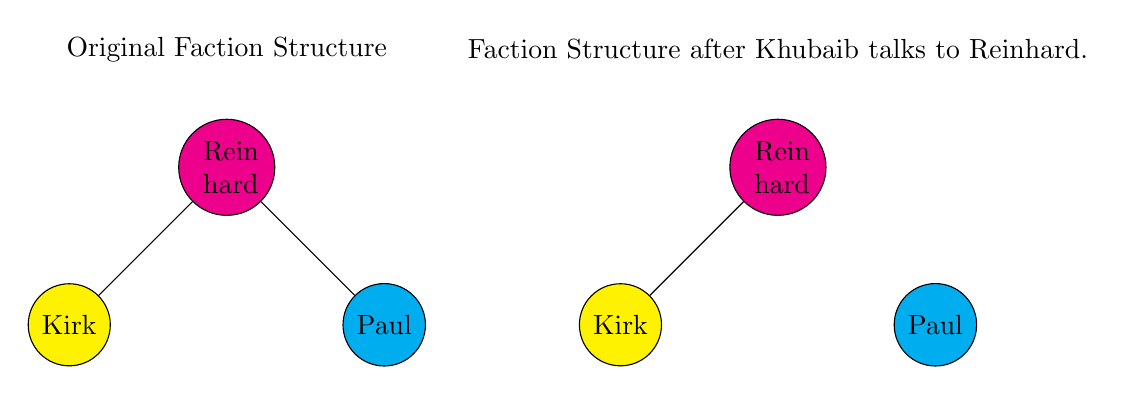
\begin{tikzpicture} 
            \node [] (L) at (2,3.5) {Original Faction Structure};
            \node [style={circle,draw, fill=yellow}] (A) at (0,0) {Kirk};
            \node [style={circle,draw,text width=6mm, fill = magenta}] (B) at (2,2) {Rein\\hard};
            \node [style={circle,draw, fill = cyan}] (C) at (4,0) {Paul};
            \draw (A) -- (B);
            \draw (B) -- (C);

            
            \node [] (L) at (9,3.5) {Faction Structure after Khubaib talks to Reinhard.};
            \node [style={circle,draw, fill = yellow}] (A1) at (7,0) {Kirk};
            \node [style={circle,draw,text width=6mm, fill = magenta}] (B1) at (9,2) {Rein\\hard};
            \node [style={circle,draw}, fill = cyan] (C1) at (11,0) {Paul};
            \draw (A1) -- (B1);


        \end{tikzpicture}
        \caption{Kirk is in alliance with Reinhard and Reinhard is in alliance with Paul. So Kirk, Reinhard and Paul form a faction. On the left we have the original faction structure then on right we have the faction structure after Khubaib talks to Reinhard and convince him to break his alliance with Paul.}
        \label{1}
    \end{figure}
        
%  \vspace{0.5cm}
\begin{figure}[!tbh]
    \centering
    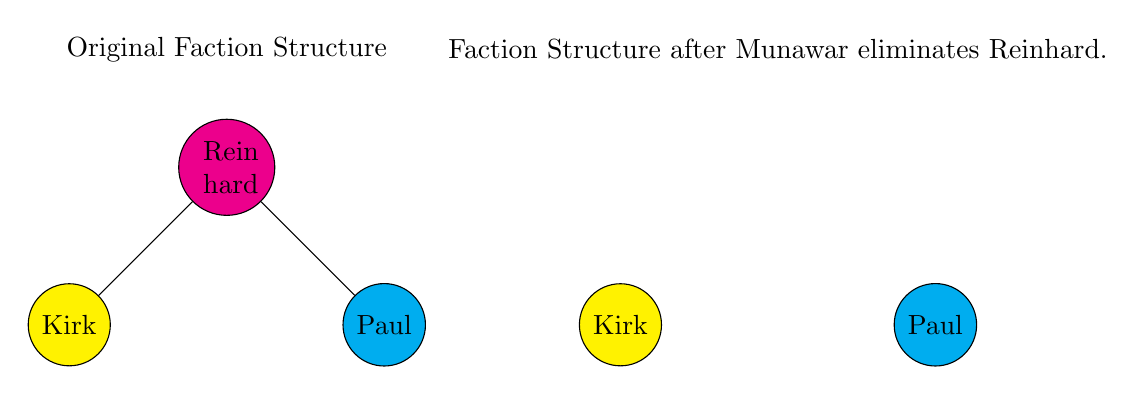
\begin{tikzpicture} 
        \node [] (L) at (2,3.5) {Original Faction Structure};
        \node [style={circle,draw, fill=yellow}] (A) at (0,0) {Kirk};
        \node [style={circle,draw,text width=6mm, fill = magenta}] (B) at (2,2) {Rein\\hard};
        \node [style={circle,draw, fill = cyan}] (C) at (4,0) {Paul};
        \draw (A) -- (B);
        \draw (B) -- (C);

        
        \node [] (L) at (9,3.5) {Faction Structure after Munawar eliminates Reinhard.};
        \node [style={circle,draw, fill = yellow}] (A1) at (7,0) {Kirk};
        \node [style={circle,draw}, fill = cyan] (C1) at (11,0) {Paul};
       


    \end{tikzpicture}
    \caption{Kirk is in alliance with Reinhard and Reinhard is in alliance with Paul. So Kirk, Reinhard and Paul form a faction. On the left we have the original faction structure then on right we have the faction structure after after Munawar eliminates Reinhard.}
    \label{2}
\end{figure}


  \question Let $G$ and $H$ be some graphs. Show that $G \cong H \iff \overline{G} \cong \overline{H}$
  \begin{solution}
    % Enter solution here 
  \end{solution}

   \question Show that a vertex $c$ in a connected simple graph $G$ is a cut vertex if and only if there are vertices $u$ and $v$, both different from $c$, such that every path between $u$ and $v$ passes through $c$.
   \begin{solution}
    % Enter solution here 
  \end{solution}


  \question For this problem, we recommend drawing out some graphs to build your intuition then give a constructive proof.
    \begin{definition}
        Let $G = (V,E)$ be a graph. A decomposition of $G$ is a list of subgraphs of $G$ (obtained from removing edges of $G$) such that each edge appears in exactly one subgraph in the list. Figure~\ref{fig:exampl_ahg} shows an example of graph decomposition.
    \end{definition}

    \begin{figure}[!tbh]
        % \vspace*{1cm}
        \begin{center}
        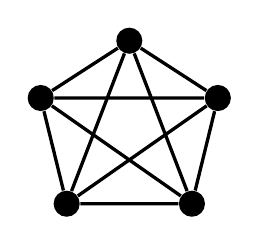
\begin{tikzpicture}[scale=.75]
            
            \node[style={fill=black,circle}] (a) at (4,1.7){};
            \node[style={fill=black,circle}] (b) at (2.5,0.73){};
            \node[style={fill=black,circle}] (c) at (2.939339828,-1.06){};
            \node[style={fill=black,circle}] (d) at (5.06066,-1.06){};
            \node[style={fill=black,circle}] (e) at (5.499,0.73){};
            \draw[black,very thick] (a)--(b) (a)--(c) (a)--(d) (a)--(e) (b)--(c) (b)--(d) (b)--(e) (c)--(d) (c)--(e) (d)--(e);
    
            \end{tikzpicture} 
            \hspace{1cm} 
\includegraphics[scale = 0.1]{right-arrow.png} \hspace{1cm}
            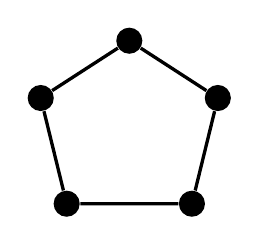
\begin{tikzpicture}[scale=.75]
            
                \node[style={fill=black,circle}] (a) at (4,1.7){};
                \node[style={fill=black,circle}] (b) at (2.5,0.73){};
                \node[style={fill=black,circle}] (c) at (2.939339828,-1.06){};
                \node[style={fill=black,circle}] (d) at (5.06066,-1.06){};
                \node[style={fill=black,circle}] (e) at (5.499,0.73){};
                \draw[black,very thick] (a)--(b) (a)--(e) (b)--(c)  (c)--(d) (d)--(e);
        
                \end{tikzpicture} 
                \hspace{1cm}
                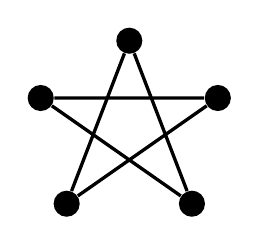
\begin{tikzpicture}[scale=.75]
            
                    \node[style={fill=black,circle}] (a) at (4,1.7){};
                    \node[style={fill=black,circle}] (b) at (2.5,0.73){};
                    \node[style={fill=black,circle}] (c) at (2.939339828,-1.06){};
                    \node[style={fill=black,circle}] (d) at (5.06066,-1.06){};
                    \node[style={fill=black,circle}] (e) at (5.499,0.73){};
                    \draw[black,very thick]  (a)--(c) (a)--(d) (b)--(d) (b)--(e) (c)--(e) ;
            
                    \end{tikzpicture} 
        \end{center}
            \caption{An example of decomposition of $K_5$ into two $C_5$s.}  
            \label{fig:exampl_ahg}     
    \end{figure}
    
    Prove that for any $n\in \mathbb{Z}^+\setminus\{1,2\}$ the graph $K_n$ can be decomposed into three isomorphic subgraphs if and only if $n+1$ is not divisible by 3. 
    \begin{solution}
        % Enter solution here
    \end{solution}


    \question In the film Good Will Hunting, a ``difficult'' math problem that Matt Damon's character Will Hunting is seen solving is the following:

    Draw all possible 10 vertices tree that have no vertex of degree 2. 

    But it turns out this problem is not so difficult after all. Solve the problem from Good Will Hunting.

    \begin{figure}[!tbh]
      \centering
      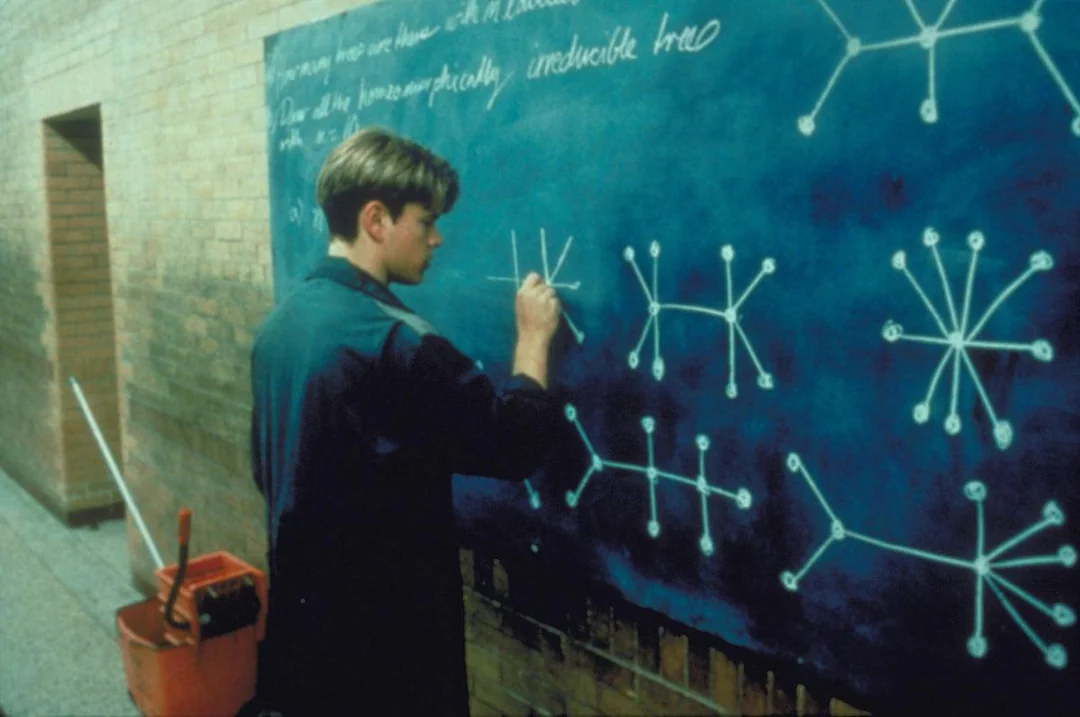
\includegraphics[scale = 0.25]{goodwillhunting.png}
      \caption{Will Hunting solving the problem, you can build on the partial solution visible on the here.}
    \end{figure}
    \begin{solution}
        % Enter solution here
    \end{solution}


\end{questions}


\end{document}

%%% Local Variables:
%%% mode: latex
%%% TeX-master: t
%%% End:
